\chapter{Optimization}
The optimization problem is a computational problem in which the objective is to find the best of all possible solutions. Deep neural networks is a form of an optimization problem to find the best possible set of weights in order to reduce the error in a network.

\noindent A generic form of an optimization problem is given by 
\begin{align}
  \begin{matrix}
    \underset{x}{\text{minimize/maximize}} &f(x) & \\
    \text{subject to} &g_i(x) \leq 0, \, \, & i=1,\dots,m \\
    &h_j(x) = 0, & j=1,\dots,p
  \end{matrix}
  \label{eq:optimization_problem}
\end{align} 
\noindent where \\
\indent $f: \mathbb{R}^n \rightarrow \mathbb{R}$ is the objective/loss function to be minimised,\\
\indent $g_i(x) \leq 0$ are called inequality constraints,\\
\indent $h_j(x) = 0$ are called equality constraints, and \\
\indent $m\geq0$ and $p\geq0$
\noindent If $m=p=0$, the problem is an unconstrained optimization problem.
\subsubsection*{Minimum/Maximum Point}
Let $x^*$  be points of the function $f(x)$ defined in (\ref{eq:optimization_problem}) and $u \in \mathbb{N}(x^*,\delta)$ where $\mathbb{N}$ is a $\delta$-neighbourhood of $x^*$. Then, $x^*$ is said to be a
\begin{enumerate}[(i)]
    \item local minimum if $f(x^*) < f(u)$    $\forall u\in\mathbb{N}$
    \item local  maximum if $f(x^*) > f(u)$ $\forall u\in\mathbb{N}$
    \item global minimum if $f(x^*) < f(u)$ $\forall u\in\mathbb{R}$
    \item global maximum if $f(x^*) > f(u)$ $\forall u\in\mathbb{R}$
\end{enumerate}

\begin{figure}[ht]
    \centering
    \includegraphics[scale=0.70]{CHAPTER_3/c3_fig_min_max_draw.png}
    \caption{Minimum and Maximum points}
    \label{fig:min_max_illustration}
\end{figure}
\subsubsection*{Determining Minimum/Maximum Point}
For a function $f(\textbf{x})$ where $\textbf{x} = (x_1,x_2. \dots, x_n) \in \mathbb{R}^n$, the condition for the presence of a stationary point (minimum or maximum point) is given by
\begin{align}
    \label{eq:grad_f_x}
    \textbf{G} = \nabla f \begin{pmatrix}
        \dfrac{\partial f}{\partial x_1} & \dfrac{\partial f}{\partial x_2} & \dots , \dfrac{\partial f}{\partial x_n}
    \end{pmatrix} = \textbf{0}
\end{align}
The second derivative of $f(x)$ is given by the Hessian matrix, $\textbf{H}$
\begin{align}
    \label{eq:Hessian_matrix}
    \textbf{H} = \begin{bmatrix}
        \dfrac{\partial^2 f}{\partial x_1^2} & \dfrac{\partial^2 f}{\partial x_1 \partial x_2} & \dots & \dfrac{\partial^2 f}{\partial x_1 \partial x_n} \\
        \dfrac{\partial^2 f}{\partial x_2\partial x_1} & \dfrac{\partial^2 f}{\partial x_2^2} & \dots & \dfrac{\partial^2 f}{\partial x_2 \partial x_n} \\
        \vdots & \vdots & \ddots & \vdots \\
        \dfrac{\partial^2 f}{\partial x_n\partial x_1} & \dfrac{\partial^2 f}{\partial x_n \partial x_2} & \dots & \dfrac{\partial^2 f}{\partial x_n^n}
    \end{bmatrix}
\end{align}
The nature of the stationary points of $f(x)$ can be determined by studying the positive definiteness of (\ref{eq:Hessian_matrix}) using its eigenvalues. If all the eigenvalues of $\textbf{H}$ are positive, then $\textbf{H}$ is symmetric positive definite, indicating the presence of a \textbf{local minimum}.
\section{Optimization algorithms}
The solutions to the optimization problem are vital in modern machine learning and artificial intelligence algorithms, which includes weight optimization in deep learning. There are a number of popular optimization algorithm currently developed to solve the problem. Hence, choosing the right algorithm can be challenging as well.
%\subsubsection*{Network Error}
Let the network cost function, $c$, be given by the squared difference between the predicted value and the true value:
\begin{align}
   c = \dfrac{1}{2n}\sum^{n}_i (\widehat{y_i}-y_i)^2
  \label{network_error}
\end{align}
where $n$ is the total number of input.\\
\noindent The difference is squared to avoid the sum of errors of multiple input vector to be zero which can mislead the network to have perfect predictive power. The goal of the network is to adjust the weight to reduce the network error as much as possible. The idea of reducing a function to a value is synonymous to (\refeq{eq:optimization_problem}) an optimization problem. The network error in (\refeq{network_error}) is a quadratic equation in this case.
\begin{figure}[H]
  \centering
  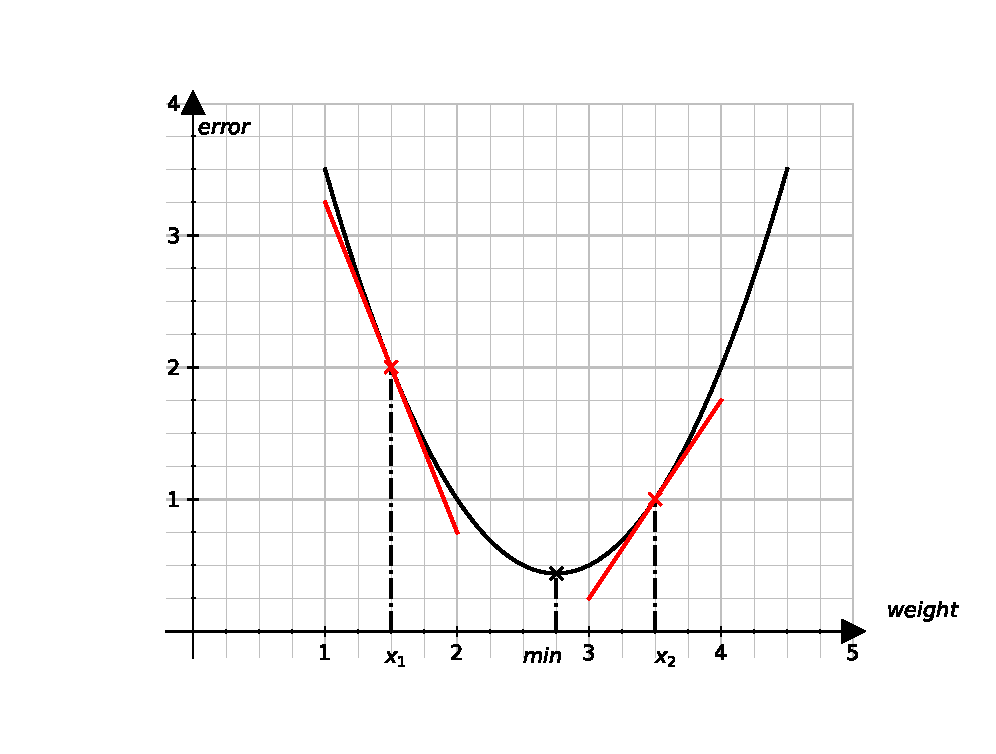
\includegraphics[scale=0.75]{CHAPTER_2/c2_fig_network_error_python.eps}
  \caption{Network Error over different weight}
  \label{network_error_graph}
\end{figure}
\noindent Figure (\ref*{network_error_graph}) is a graphical representation of the network error function. Our goal is to reach the minimum of the function by adjusting the weight value.
\subsection*{Gradient Descent}
In order to reach the bottom of the function; we need to adjust the weight such that the derivative of the error function is 0. The approach of updating the weight based on the gradient of the error function is known as \textbf{gradient descent}. The derivative with respect to the weights of the network error (\refeq{network_error}) for a single input is given by
\begin{align}
  \frac{\partial e}{\partial w_{ij}} = (\widehat{y_i}-y_i)\frac{\partial \widehat{y_i}}{\partial w_{ij}}
  \label{derivative_network_error}
\end{align}
From figure (\refeq{network_error_graph}); we can observe that if the gradient is negative then we have underestimated the predicted value and need to increase the weight to reach the optimal value. On the other hand, if the gradient is positive then we have overestimated the predicted value and need to decrease the weight to reach the optimal value. The equation (\refeq{derivative_network_error}) provides us with the opposite direction and amount to adjust the weight. Hence, the update rule of the weights for gradient descent method is given by
\begin{align}
  w_{ij}^{t+1} = w_{ij}^{t} - \dfrac{de}{dw_{ij}}
\end{align}
In the gradient descent method, the network learns from the gradient of the error function and adjust the weights accordingly to reduce the error. However, the gradient alone can be quite large, causing oscillations as we go down the error function. This problem by introducing a \textbf{learning rate} $\alpha$ prior to adjusting the weight.
\subsubsection*{Learning Rate}
The learning rate is typically denoted by the Greek letter alpha $\alpha$. It helps the network to control the rate at which the weights are changing. Having a system with a high learning rate may lead to an oscillating network when trying to find the optimal weight and having a slow learning rate increases the number of iterations required when optimizing the network. The adjusted update rule of the weight is given by
\begin{align}
  w_{ij}^{t+1} = w_{ij}^{t} - \alpha\dfrac{\partial e}{\partial w_{ij}}
\end{align}
where $\alpha \in (0,1)$
\subsection*{Stochastic Gradient Descent}
The Stochastic Gradient Descent dates back to the Robbins-Monro algorithm from the 1950s and is still an important optimization algorithm \cite{Robbins1951}. Instead of adjusting the weight to the average loss function, we can approximate the gradient by only one random directional derivative of the error. Thus, the number of computation in the gradient descent method can be significantly reduced by a factor of $n$ (where $n$ is the number of direction). The stochastic gradient method (SGM) is given by 
\begin{align}
    \label{eq:SGM_def}
    w^{t+1} = w^{t} - \alpha_t {(\nabla e)}_i
\end{align}
where $\alpha_t$ is the learning rate at the $t^{th}$ iteration which may vary with iterations.\\
As we move closer to the bottom of the minimum of the function; the solution starts to oscillate since we are moving the weight in random directions. Thus, the learning rate should be reduced gradually as we iterate. Some commonly used reduction of learning rate is given by 
\begin{align}
    \label{eq: learning_rates}
        \eta(t) &= \eta_i \,\,\, \,\,\,\, \text{ if } t_i \leq t \leq t_{i+1} &\text{piecewise constant} \\
        \eta(t) &= \eta_0e^{-\lambda t} &\text{exponential decay} \\
        \eta(t) & = \eta_0 (\beta t + 1)^{-\alpha} &\text{polynomial decay}
\end{align}
where $\lambda$, $\beta$, and $\alpha$ are known as hyperparameter. \\
Training dataset can be very large in certain cases which leads to a greater cost of compute at each iteration for the gradient descent, so stochastic gradient descent is preferred in these cases.
\subsection*{Mini-Batch Stochastic Gradient Descent}
In order to make use of the features of both gradient descent and stochastic gradient descent; we introduce the mini-batch stochastic gradient descent. In this approach, instead of iterating in the direction of the full gradient or only in one direction of the full gradient, we split the dataset into small batches and compute the gradient of each batch. The formula of the stochastic gradient descent is given by 
\begin{align}
    \label{mb-sgd}
    \textbf{w}^{t+1} &= \textbf{w}^{t} - \eta_t \textbf{g}_t \\
    \nonumber
    \textbf{g}_t &= \nabla_{\mathcal{B}_t}e(\textbf{x},\textbf{w}) 
\end{align}
where $\mathcal{B}_t$ is a mini-batch of elements drawn uniformly at random from the training set (the expectation of the gradient remains unchanged). \\ Since we are using a mini-batch, the updates are closer to the full gradient but at a reduced cost.
\subsection*{Newton's Method}
For minimizing $f(x)$, $x \in \mathbb{R}$, we need to solve $g(x) = e^{'}(x)=0$. Newton's iteration is given by 
\begin{align}
  x_{n+1} &= x_{n} - \dfrac{g(x_{}n)}{g^{'}(x_n)} \\
          &= x_{n} - \dfrac{f^{'}(x_{}n)}{f^{''}(x_n)}
\end{align}
For multivariate functions we need to minimise $f(\mathbf{x})$ over $\mathbf{x} \in \mathbb{R}^n$, that it
\begin{align}
  \begin{matrix}
    \underset{\mathbf{x}\in\mathbb{R}^n}{min} f(\mathbf{x}), & \,\,\, \mathbf{x} =(x_1,x_2,\dots,x_n)^T \in \mathbb{R}^n
  \end{matrix} 
\end{align}
The Newton's iteration for multivariate function is given by
\begin{align}
  \mathbf{x_{n+1}} = \mathbf{x_{n}} - H(\mathbf{x_n})^{-1}\nabla f(\mathbf{x_n})
\end{align}
where $H(\mathbf{x_n})$ is the Hessian matrix of $f(\mathbf{x})$.\\
\noindent We can observe from (\refeq{eq:Hessian_matrix}) that calculating the inverse of the Hessian matrix can be computationally very expensive for higher dimensions. Replacing $H(\mathbf{x_n})^{-1}$ by $\alpha \mathcal{I}$ where $\mathcal{I}$ is the identity matrix; we get the \textbf{method of steepest descent} given by
\begin{align}
  \mathbf{x_{n+1}} = \mathbf{x_{n}} - \alpha \textbf{I} \nabla f(\mathbf{x_n})
\end{align}
where $\alpha \in (0,1)$
\subsection*{Momentum}
%https://ui.adsabs.harvard.edu/abs/1986Natur.323..533R/abstract
%Documention on when momentum first appeared
\subsubsection*{Exponentially Weighted Moving Average}
The exponentially weighed moving average (EWMA), also known as exponential moving average (EMA), of a series of data points $S_t$ is given by 
\begin{align}
    \label{eq:ewma_def}
    \mu_t &= \beta \mu_{t-1} + (1-\beta)S_t \\
    \nonumber
    \mu_0 &= c
\end{align}
where $c \in \mathbb{R}$ and $\beta \in (0,1)$ is known as the smoothing constant. $\beta$ represents the weightage that is going to be assigned to the past values. The average number of previous reading is approximately given by $n={(1-\beta)}^{-1}$. The higher the value of $\beta$ the greater the number of points we average over.
\subsubsection*{SGD with Momentum}
The momentum method was mentioned in Rumelhart, Hinton and Williams' paper on back-propagation learning in 1986 \cite{Rumelhart:1986aa}.  From the SGD, it was observed that the weight update can be very noisy. In order to smoothen the search direction in the SGD, an exponentially moving average is implemented on the gradient. The SGD with momentum can be written in the form
\begin{align}
    \label{eq: SGF_with_momentum}
    \textbf{w}^{t+1} &= \textbf{w}^{t} - \eta \boldsymbol{\mu}^t
    \intertext{where the exponential moving average of the gradient is given by}
    \nonumber
    \boldsymbol{\mu}^{t} &= \beta \boldsymbol{\mu}^{t-1} + (1-\beta)\nabla(e)^t \\
    \nonumber
    \boldsymbol{\mu}_0 &= \textbf{c}
\end{align}
\subsection*{RMSProp}
%https://www.scirp.org/(S(czeh2tfqyw2orz553k1w0r45))/reference/ReferencesPapers.aspx?ReferenceID=1911091
Proposed by Geoffrey Hinton in lecture 6 of the online course "Neural Network for Machine Learning" \cite{Hinton2012}, the Root Mean Square Propagation (RMSProp) algorithm alleviates undesirable fluctuations when adjusting the weight during optimization. RMSProp is an adaptive learning rate. The idea is to reduce the step size at very large gradient to avoid fluctuations and increase the step size at smaller gradient to move steadily in the correct direction of the optimal solution; hence an adaptive learning rate at each iteration. The equations for the RMSProp is given by 
\begin{align}
    \nonumber
    \label{eq:RMSProp_def}
    {S}^t_i &= \gamma {S}^{t-1}_i + (1-\gamma)(\nabla e^t)_i^2 \\
    {w}^{t+1}_i &= {w}^t_i - \dfrac{\eta}{\sqrt{S^t_i} + \epsilon}(\nabla e^t)_i
\end{align}
where $\epsilon \approx 10^{-6}$ to ensure that we avoid dividing by zero during iterations.
\subsection*{Adam}
%https://arxiv.org/abs/1412.6980
The Adam algorithm (Adaptive Moment Estimation algorithm) is a robust update rule for the weight optimization \cite{Kingma2014}. The algorithm combines the benefits of momentum (\refeq{eq: SGF_with_momentum}) and RMSProp (\refeq{eq:RMSProp_def}). Adam is the most popular generalized algorithm performs very well in many cases. It is considered as a state-of-the-art algorithm for deep neural network optimization. The set of equations for the Adam algorithm is given by
\begin{align}
    \nonumber
    \mu^{(t)}_i &= \beta_1 {\mu}^{(t-1)}_i + (1-\beta_1)\nabla(e^{(t)})_i &\text{Momentum} \\
    \nonumber
    {S}^{(t)}_i &= \beta_2 {S}^{(t-1)}_i + (1-\beta_2)(\nabla e^{(t)})_i^2 &\text{RMSProp}    
\end{align}
To prevent $S^t$ and $\mu^t$ from becoming zero during the initial steps, a bias correction is introduced, such that
\begin{align*}
    \hat{\mu^{(t)}} = \dfrac{\mu^{t}}{1-\beta_1^t} & & \hat{S^{(t)}} = \dfrac{S^t}{1-\beta_2^t}
\end{align*}
Finally, the update rule is given by
\begin{align}
    \label{eq:Adam_def}
    {w}^{(t+1)}_i &= {w}^{(t)}_i - \dfrac{\eta}{\sqrt{S^t_i} + \epsilon}\mu_i
\end{align}
The parameters $\beta_1$, $\beta_2$ and $\epsilon$ are knows are the hyperparameters of the Adam algorithm. A common set of values that works well in literature are $\beta_1 = 0.9$, $\beta_2 = 0.9999$ and $\epsilon = 10^{-8}$ \cite{Kingma2014}.
%https://arxiv.org/pdf/1412.6980.pdf
\section{Backpropagation using Adam}
The Adam algorithm for optimization can be introduced in the weight update when training deep neural network. The problem of finding the right set of weights and biases for a deep neural network can be reduced to an optimization problem same as we defined in (\refeq{network_error}). After finding the gradients through the backpropagation algorithm, the set of updates proposed in the Adam algorithm are used to update the weights and biases in the neural network.
\begin{algorithm}[H]
  \caption{Backpropagation using Adam optimization with $n$ total number of inputs for $N$ epochs}\label{alg:back_propagation_adam_algo}
  \begin{algorithmic}[1]
  \State{\textbf{Start}}
  \For{$t = 1,2, \dots, N$}
  \For{$s = 1,2, \dots, n$}
  \State Compute the activation layer $a^{(1)}$ using $n$ input values in a batch
  \State $a^{(1)} = \sigma(w^{(1)}x + b^{(1)} )$
  \State Feed forward the $n$ input to the next layers
  \For{$l = 2,3,\dots,L$}
    \State{$z^{(l)} = w^{(l)}a^{(l-1)}+b^{(l)}$}
    \State $a^{(l)} = \sigma(z^{(l)})$
  \EndFor  
\EndFor
  \State Compute the average cost function, $C$, at the output layer $L$
  \State $c^{(t)} = \dfrac{1}{2n}\sum^{n}_s (\widehat{y_s}-y_s)^2$
  \State Compute the rate of change of the cost function $w.r.t$ to $z^{(L)}$
  \State $\delta^{(L)} = \nabla_{a^{(L)}}C \odot \sigma^{'}(z^{(L)})$
  \For{$l = L-1, L-2, \dots, 2$} 
    \State Computing the gradients
    \State $\delta^{(l)} = (w^{(l+1)})^T\sigma^{(l+1)} \odot \sigma^{'}(z^{(l)})$
    \State $\nabla_{b^{(l)}} C = \delta^{(l)}$
    \State $\nabla_{w^{(l)}} C = \delta^{(l)}a^{(l-1)}$\\
    \State Bias update
    \State $\mu^{(t)}_i = \beta_1 {\mu}^{(t-1)}_i + (1-\beta_1)\delta^{(l)}_i$
    \State ${S}^{(t)}_i = \beta_2 {S}^{(t-1)}_i + (1-\beta_2)(\delta^{(l)}_i)^2$
    \State $\hat{\mu^{(t)}} = \dfrac{\mu^{t}}{1-\beta_1^t}$
    \State $ \hat{S^{(t)}} = \dfrac{S^t}{1-\beta_2^t}$
    \State ${b}^{(t+1)}_i = {b}^{(t)}_i - \dfrac{\eta}{\sqrt{S^t_i} + \epsilon}\mu_i$\\
    \State Weight update
    \State $\mu^{(t)}_i = \beta_1 {\mu}^{(t-1)}_i + (1-\beta_1)\delta^{(l)}a^{(l-1)}_i$
    \State ${S}^{(t)}_i = \beta_2 {S}^{(t-1)}_i + (1-\beta_2)(\delta^{(l)}a^{(l-1)}_i)^2$
    \State $\hat{\mu^{(t)}} = \dfrac{\mu^{t}}{1-\beta_1^t}$
    \State $\hat{S^{(t)}} = \dfrac{S^t}{1-\beta_2^t}$
    \State ${w}^{(t+1)}_{ij} = {w}^{(t)}_{ij} - \dfrac{\eta}{\sqrt{S^t_i} + \epsilon}\mu_i$
  \EndFor
\EndFor
\end{algorithmic}
\end{algorithm}